\begin{figure}[htbp]
\centering 
  \subfloat[Box plot \acs{SCT}.]{
	  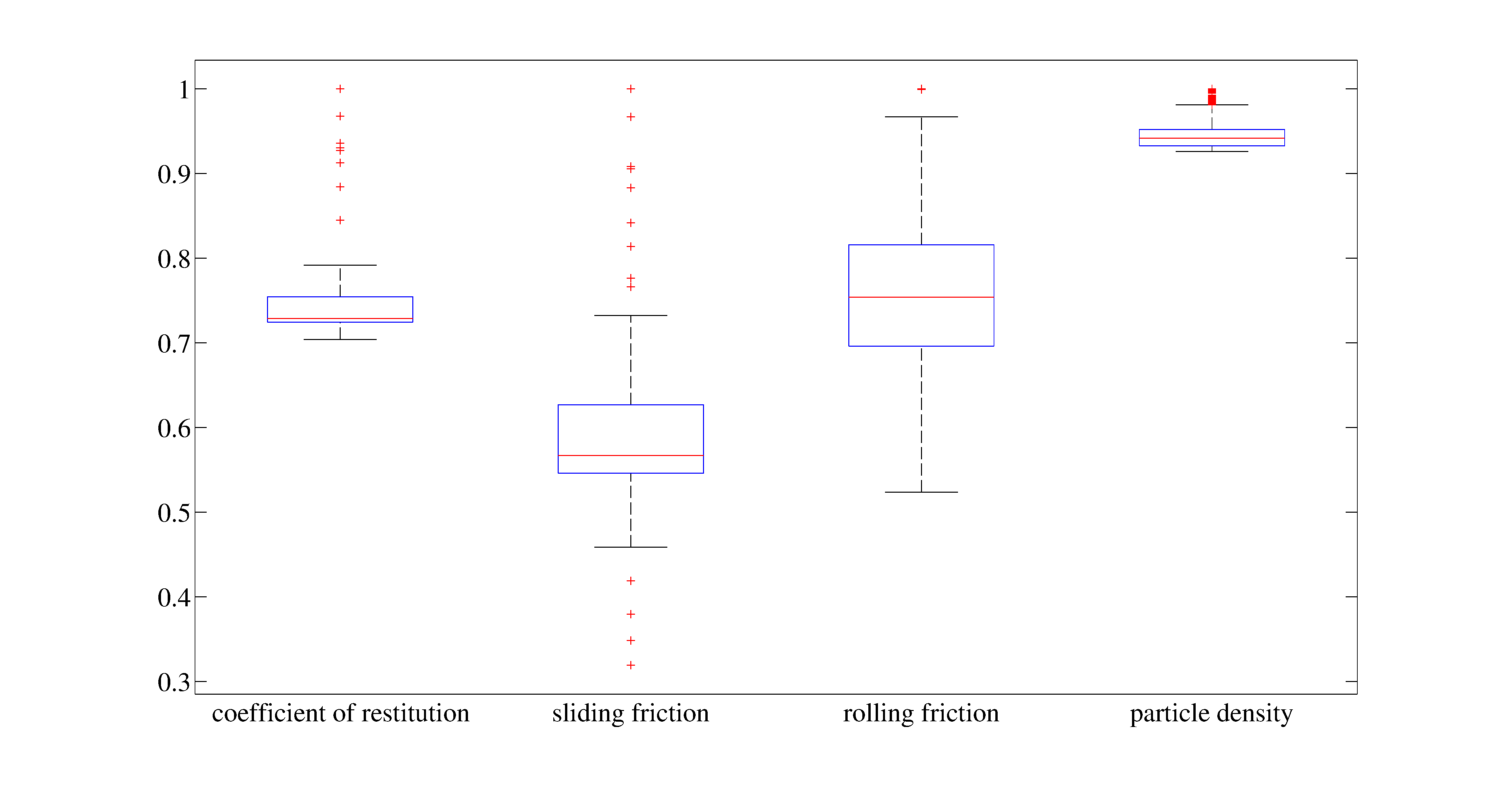
\includegraphics[width=.47\columnwidth]{images/163BoxSCTsintercoarsetest01coeffP1}
	  \label{fig:163BoxSCTsintercoarsetest01coeffP1}
  }
  \quad
  \subfloat[Density plot \acs{SCT}.]{
	  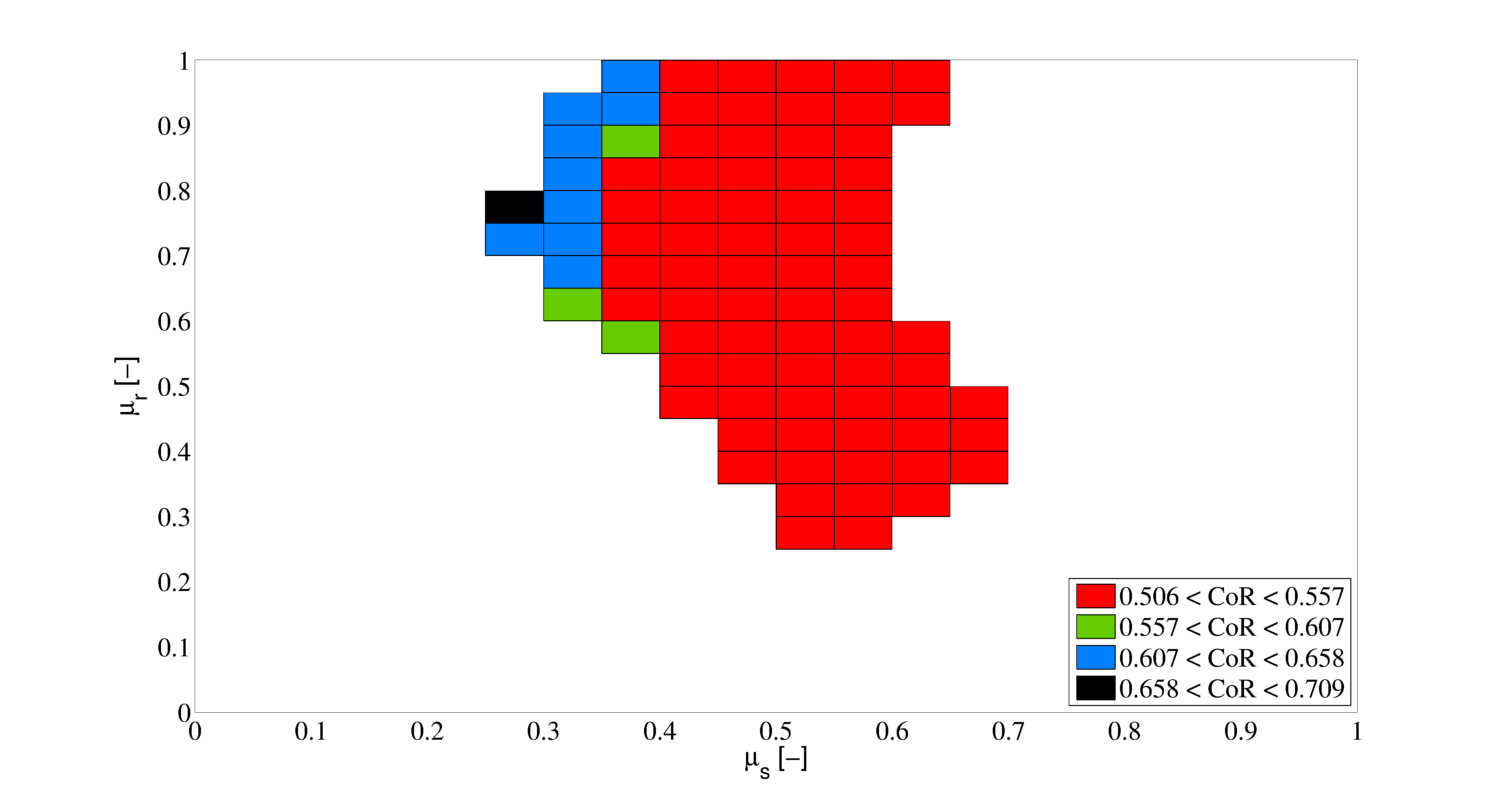
\includegraphics[width=.47\columnwidth]{images/176ileSCTsintercoarsetest02coeffP1}
	  \label{fig:176ileSCTsintercoarsetest02coeffP1}
  }
  \\
    \subfloat[Box plot \acs{AoR}.]{
	  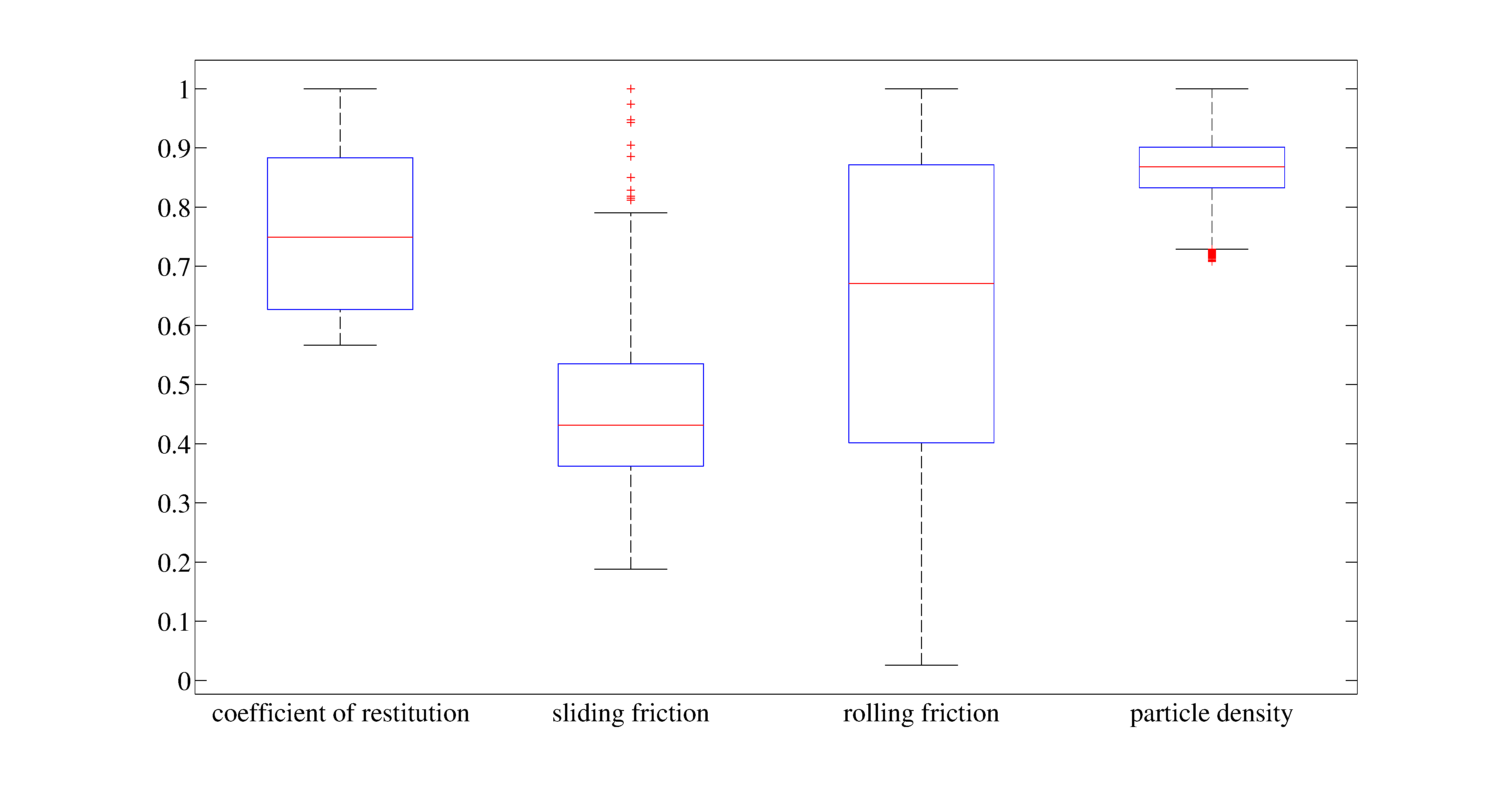
\includegraphics[width=.47\columnwidth]{images/189BoxAORsintercoarse}
	  \label{fig:189BoxAORsintercoarse}  }
  \quad
  \subfloat[Density plot \acs{AoR}.]{
	  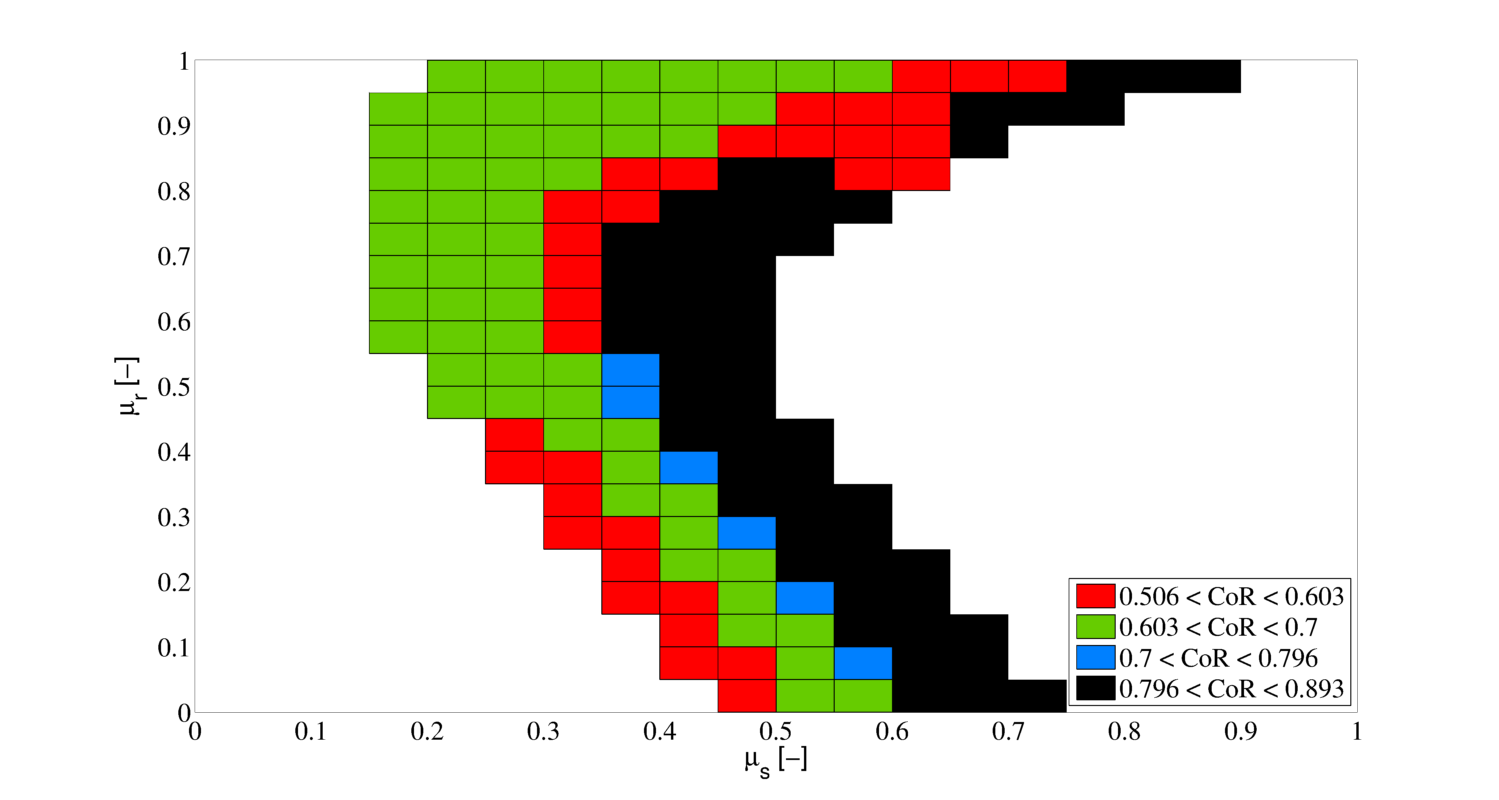
\includegraphics[width=.47\columnwidth]{images/190TileAORsintercoarse}
	  \label{fig:190TileAORsintercoarse}  }
  \\
  \subfloat[Box plot intersection: \acs{AoR} \& \acs{SCT}.]{
	  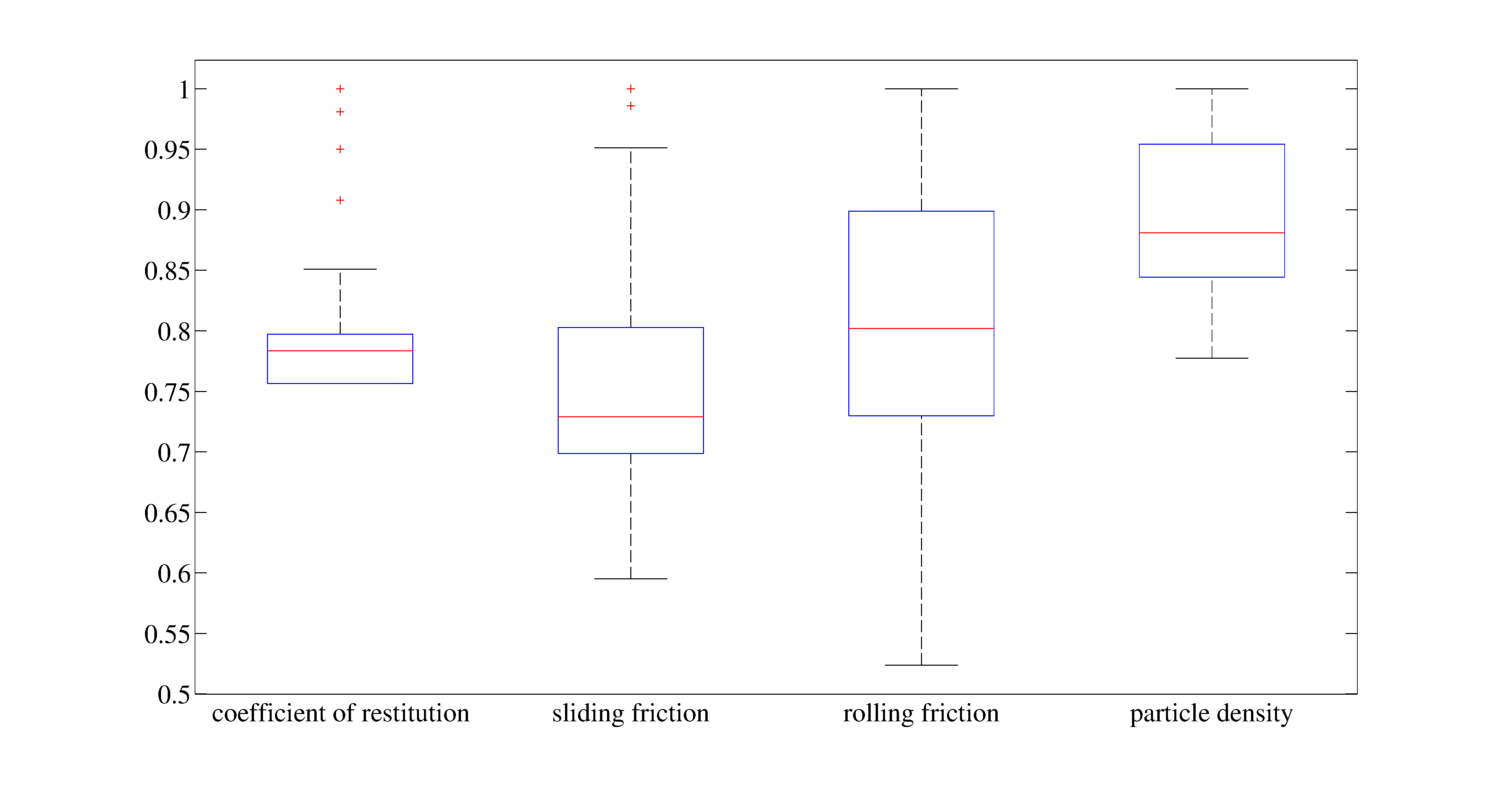
\includegraphics[width=.47\columnwidth]{images/203BoxMixsintercoarse_31}
	  \label{fig:203BoxMixsintercoarse_31}
  }
  \quad
  \subfloat[Density plot intersection: \acs{AoR} \& \acs{SCT}.]{
	  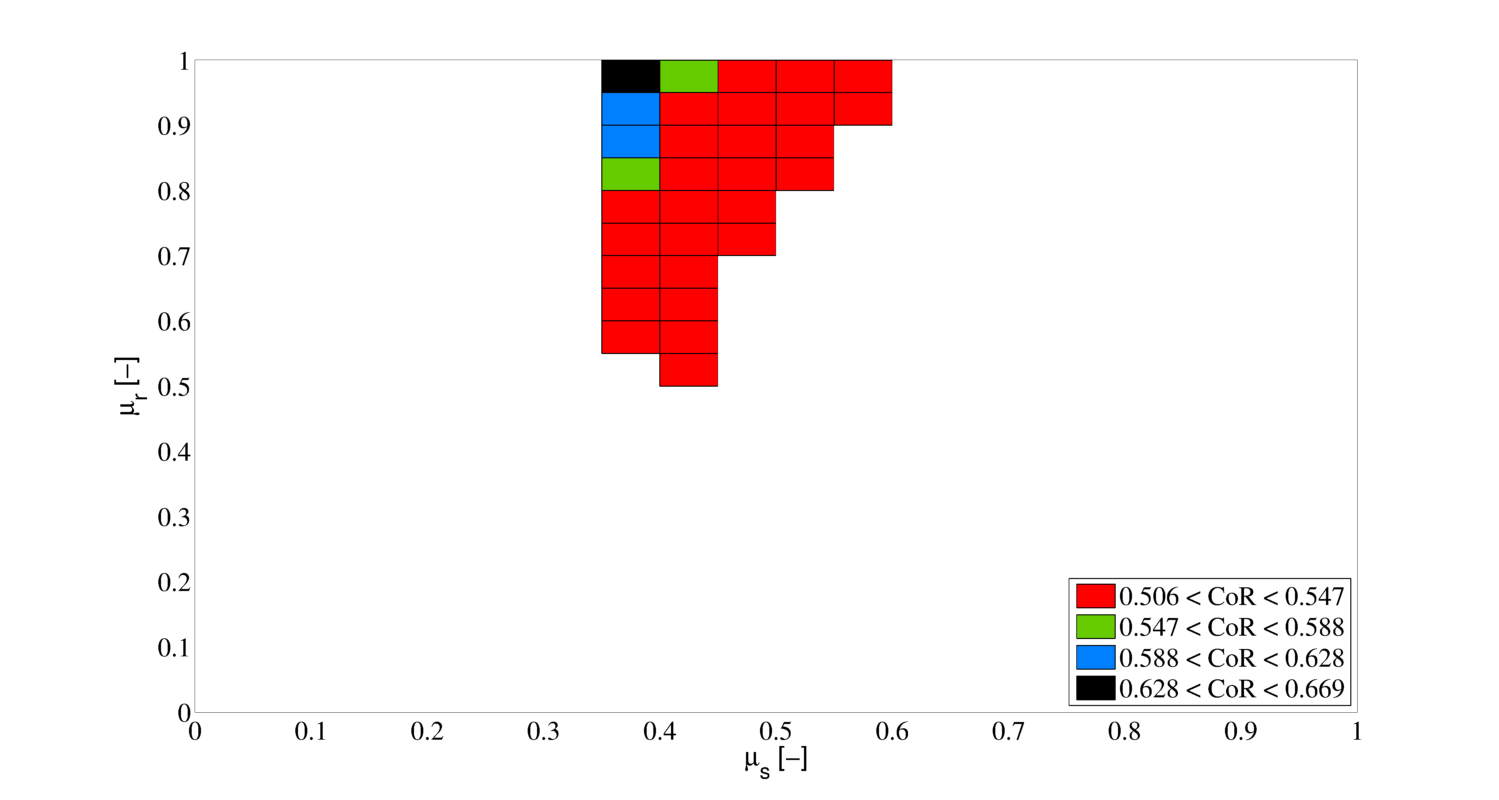
\includegraphics[width=.47\columnwidth]{images/204TileMixsintercoarse_31}
	  \label{fig:204TileMixsintercoarse_31}
  }
  \\    
  \caption[Sinter coarse valid values]{Sinter coarse valid values. The
  valid values for the \acs{SCT} and \acs{AoR} tests are shown, together with the merge values, valid for both.
  The plots referring to the single test show reasonably narrow confidence
  ranges, while Fig. \ref{fig:203BoxMixsintercoarse_31} shows unreasonably large
  valid ranges. See Section \ref{sec:remainingmaterialscharacterization} for
  the interpretation.}
  \label{fig:221boxplotssintercoarse}
\end{figure}